\documentclass[FrontPage]{grattan}
% Nothing to see here.

% Comments are deployed by the % sign; everything after % is ignored by the compiler.
% Please do not put comments before \documentclass as these are reserved for TeX directives.

% add_to_dictionary: GrattanFrameBox

\makeatletter
\newcommand{\@addboxcaption}[1]{%
\captionsetup{labelfont={bf,Orange},font={bf,Orange},format=plain,justification=raggedright,singlelinecheck=false, skip=0ex, position=above}
\caption*{#1}
\captionsetup{format=plain,font={small,bf,theGrey},labelfont={small,bf,theGrey}, position=above, skip=0pt}
}

\let\addboxcaption\@addboxcaption

\newenvironment{addsmallbox}[3][htb]{%
\setlength{\currentparskip}{\parskip}% save the value
\begin{boxe}[#1]
\begin{minipage}{\linewidth}
\begin{mdframed}[style=GrattanFrameBox]%
\setlength{\parskip}{\currentparskip} % restore the value
\@addboxcaption{#2\label{#3}}
\RaggedRight
}{\end{mdframed}\end{minipage}\end{boxe}}

\makeatother


\addbibresource{bib/Grattan-Master-Bibliography.bib}

\author{Peter Goss and Julie Sonnemann}
\title{Engaging students: creating classrooms that improve learning}

\hypersetup{pdfinfo={
Title={Engaging students: creating classrooms that improve learning},
Author={Peter Goss and Julie Sonnemann and Kate Griffiths}
}}

\GrattanReportNumber{2017-01}

% add_to_dictionary: htpb Carnellor Cain McCombs Noddings Galton with-it-ness Clearinghouse Seligman PERMA TEMAG 
% add_to_dictionary: Marzano
% add_to_dictionary: preservice TALIS PBL ABA PBIS htbp
% add_to_dictionary: Wheldall Beaman
% add_to_dictionary: Dunson ICSEA
% stop_if_present: diffuse
% add_to_dictionary: 

% editorial_author_only: Carmela Chivers

\acknowledgements{%
This report was written by Peter Goss, Julie Sonnemann, and Kate Griffiths. Carmela Chivers made substantial contributions to the report.


We would like to thank the members of Grattan Institute's School Education Program Reference Group for their helpful comments, as well as numerous government and industry participants and officials for their input.

The opinions in this report are those of the authors and do not necessarily represent the views of Grattan Institute's founding members, affiliates, individual board members reference group members or reviewers.
Any remaining errors or omissions are the responsibility of the authors.

Grattan Institute is an independent think-tank focused on Australian public policy.
Our work is independent, practical and rigorous.
We aim to improve policy outcomes by engaging with both decision-makers and the community.

For further information on the Institute's programs, or to join our mailing list, please go to: \textcolor{blue}{\url{http://www.grattan.edu.au/}}.

{\footnotesize
This report may be cited as:
Goss, P., Sonnemann, J., and Griffiths, K\@. (2017). \emph{\mytitle}. Grattan Institute.

ISBN: 978-1-925015-98-0

All material published or otherwise created by Grattan Institute is licensed under a Creative Commons Attribution-NonCommercial-ShareAlike 3.0 Unported License\par
}
}

\begin{document}


\begin{overview}
When students are engaged in class, they learn more. It is vital that teachers create the right classroom climate for learning: raising student expectations; developing a rapport with students; establishing routines; challenging students to participate and take risks. These all affect how much their students engage and learn.
 
In Australia, many students are consistently disengaged in class: as many as 40 per cent are unproductive in a given year. The main problem is not aggressive and anti-social behaviour. More prevalent and stressful for teachers are minor disruptions, such as students talking back. Nor is it just about noise: nearly one in four students are compliant but quietly disengaged. 
 
We do not know exactly what causes students in Australia to disengage – it could be problems at home, or subject matter that is too hard or too easy, or poor-quality teaching. But we do know disengagement matters. Disengaged students are one to two years behind their peers. Students who are quietly disengaged do just as badly as those acting out, and disruptive behaviour also reduces how much other students learn.
 
Teachers are calling for more support on classroom strategies. New teachers rate handling difficult student behaviours as their top professional challenge – and most feel under-prepared by their training. Even teachers with years of experience struggle. Nearly one third of all teachers are highly stressed by the challenges of engaging and re-engaging students in class. This can become a downward spiral, where poor teacher responses disrupt the class and lead to more students disengaging. 
 
Overcoming student disengagement is complicated. What is taught and the way it is taught are crucial. But creating a good learning environment in the classroom is necessary too.
 
This report calls for policy reforms to build teacher capabilities to improve classrooms. It avoids simplistic calls for ‘old-fashioned discipline’, but it also acknowledges that compelling content is not enough on its own. 
 
Teachers must first know what strategies and approaches work best in the classroom. This means Australia’s initial teacher education courses need to focus more on evidence-based techniques. Teachers then need to learn how to create the right learning climate, and how to respond well in the heat of the moment. 
 
School leaders must go beyond creating a school-wide behaviour plan. They must also provide practical support for teachers, with opportunities for collaboration, observation and feedback, which are especially important for developing these nuanced classroom skills. And governments should direct more support to disadvantaged schools where student engagement is weakest.

Implementing these recommendations will help create a better learning environment in every Australian classroom, so that every child can reach their learning potential.
\end{overview}

\begin{recommendations}\label{chap:recommendations}\raggedright%
\addsec{School-level recommendations}\label{sec:recommendation-1-school-level}
\subsubsection{A school-wide behaviour management plan is not enough}\label{subsubsec:school-wide-behaviour-management-plan}

\begin{itemize}
    \item A school-wide behaviour management plan is essential, but not enough. Schools should also build teacher capabilities to pro-actively create effective classroom environments.
\end{itemize}

\subsubsection{Provide all teachers with practical support to improve the classroom climate for learning}\label{subsubsec:provide-all-teachers-practical-support}

\begin{itemize}
    \item Strengthen induction programs for all beginning teachers, and ensure they are led by expert mentors. 
    \item Provide \emph{all} teachers with regular opportunities to collaborate with their colleagues and to give and receive feedback on how to improve the classroom climate for learning.
    \item Provide practical tools to help teachers:
    \begin{itemize}
        \item engage their classes, such as student response cards
        \item identify triggers for student disengagement so they can adapt and improve their approaches.
    \end{itemize}
\end{itemize}

%Julie!!! - change bullet points? To make a bullet point under a bullet point you need: 
    %\begin{itemize}
    %\item bullet #1.
        %\begin{itemize}
            %\item bullet #2
        %\end{itemize}
    %\end{itemize}

\vfill
\columnbreak  % HP: This is better.

\addsec{System-level recommendations}\label{rec:recommendation-2-system-level}
\subsubsection{Strengthen university training for trainee teachers}\label{subsubsec:ITEs-make-classroom-environment-priority}
\begin{itemize}
    \item Government should only accredit initial teacher education courses which:
    \begin{itemize}
        \item teach evidence-based techniques for engaging and managing students, and whose graduates can demonstrate that they can apply these approaches in practice.
        \item include school placements with time in challenging classes guided by an expert mentor, as well as time at the start of the school year when expectations and routines are set.
    \end{itemize}
\end{itemize}
\subsubsection{Promote the use of evidence in classrooms}\label{subsubsec:promote-use-evidence}
\begin{itemize}
    \item Make the extensive evidence-based theory on classroom environments more accessible to schools and teachers.
    \item Invest in tools at scale that help teachers assess and improve engagement, so each school does not reinvent the wheel.
\end{itemize}

\subsubsection{Target support to struggling schools}\label{subsubsec:target-support-struggling-schools}
\begin{itemize}
    \item Target support to low socio-economic schools, where student engagement is lowest.
\end{itemize}

\subsubsection{Gather better information on why students are disengaged }\label{subsubsec:gather-better-information}
\begin{itemize}
    \item Collect better data to provide more insight into student engagement on the ground, with more nuanced indicators.

\end{itemize}

\end{recommendations}

\contentspage

\chapter{The classroom environment matters to student learning}\label{chap:classroom-environment-matters}

What teachers teach (the curriculum) and how they teach it (pedagogy) are central to the value of every lesson. But other elements of teaching matter too.
 
In this report we look at one of these `other' elements of effective teaching – creating a classroom environment that gives all students the best opportunity to learn. A good learning environment raises student expectations, encourages them to participate, and ensures that no student can fly under the radar.%
    \footcites{Evertson2006ClassroomManagementField}{Jones2004ComprehensiveClassroomManagement}{Marzano2003ClassroomManagementWorks}{McDonald2013ClassroomManagementEngaging}{Porter2007StudentBehaviourTheory}
 
Get it right, and students will thrive in the class; they may even love it. Get it wrong, and the classroom can become a place of stress, infecting the teacher and the students. 

% \setlength{\currentparskip}{\parskip}
% \begin{boxe}
% \begin{minipage}[\textheight]{\linewidth}
% \begin{mdframed}[style=GrattanFrameBox]
% \setlength{\parskip}{\currentparskip}
% \addboxcaption{How to read this report}
% \Chapref{chap:classroom-environment-matters} gives an overview of why the classroom environment matters.
% The following chapters look at today's outcomes: how much students are engaged in Australian classrooms (\Chapref{chap:many-students-disengaged}) and the challenges teachers experience in creating positive learning environments (\Chapref{chap:teachers-struggle}). \Chapref{chap:what-works-best} outlines the evidence on what works best, and how to implement it in practice. \Chapref{chap:schools-can-do-more} examines what schools can do better to improve learning environments, and \Chapref{chap:policy-reforms-essential} outlines what policy makers can do.
% \end{mdframed}
% \vfil
% \begin{mdframed}[style=GrattanFrameBox]
% \setlength{\parskip}{\currentparskip}
% \addboxcaption{How terms are used in this report}%{box:how-terms-are-used}
% In this report, `disengaged' is an umbrella term that refers to:
% \begin{itemize}[leftmargin=1em]
%     \item Passively disengaged behaviours: where a student is compliant but quietly disengaged from learning
%     \item Low-level disruptive behaviours: where a student is noisy, restless or interrupting others and disengaged in learning
%     \item Aggressive and anti-social behaviours: where a student is very uncooperative or fails to comply with classroom norms
% \end{itemize}
% These terms are visualised in the framework in \Vref{fig:students-disengage-variety-ways}.
% \end{mdframed}
% \end{minipage}
% \end{boxe}

\begin{addsmallbox}{How to read this report}{box:how-to-read-this-report}
\Chapref{chap:classroom-environment-matters} gives an overview of why the classroom environment matters.
The following chapters look at today's outcomes: how much students are engaged in Australian classrooms (\Chapref{chap:many-students-disengaged}) and the challenges teachers experience in creating positive learning environments (\Chapref{chap:teachers-struggle}). \Chapref{chap:what-works-best} outlines the evidence on what works best, and how to implement it in practice. \Chapref{chap:schools-can-do-more} examines what schools can do better to improve learning environments, and \Chapref{chap:policy-reforms-essential} outlines what policymakers can do.
\end{addsmallbox}

\begin{addsmallbox}{How terms are used in this report}{box:how-terms-are-used}
In this report, `disengaged' is an umbrella term that refers to:
\begin{itemize}[leftmargin=1em]
    \item Passively disengaged behaviours: where a student is compliant but quietly disengaged from learning
    \item Low-level disruptive behaviours: where a student is noisy, restless or interrupting others and disengaged in learning
    \item Aggressive and anti-social behaviours: where a student is very uncooperative or fails to comply with classroom norms
\end{itemize}
These terms are visualised in the framework in \Vref{fig:students-disengage-variety-ways}.
\end{addsmallbox}

\section{Classroom environments affect teachers and students}\label{sec:classroom-environments-affect-teachers-students}
At the start of every year, teachers have the opportunity to create an effective learning environment. The climate that emerges in each classroom in the first few weeks can persist for the rest of the year.%
    \footcites{Marzano2003ClassroomManagementWorks}{Rogers2015ClassroomBehaviourPractical}

The quality of the classroom environment matters, to both student well-being and academic learning. Teacher expectations, behaviours, and interactions in the classroom all affect how well the students learn.

A range of classroom environmental factors affect learning.%
    \footcites{Hattie2008visiblelearningsynthesis}{Marzano2003ClassroomManagementWorks}{Oliver2011TeacherClassroomManagement}{Simonsen2008EvidenceBasedPractices}
A major 2008 study identified interventions related to the classroom climate that significantly improved student engagement and learning.%
    \footcite{Hattie2008visiblelearningsynthesis}
It highlighted the importance of teachers being clear, setting high expectations for student achievement, and working hard to develop good relationships with and between students (see \Vref{fig:classroom-environment-factors}). 
%CHECK REF!!! Hattie 2008 or 2009??

Empirical studies consistently show that engaging and well-managed classrooms enhance student behaviour and achievement.%
    \footnote{\textcites{Marzano2003ClassroomManagementWorks}{Oliver2011TeacherClassroomManagement} -- effect sizes are: 0.71 for student behaviour, 0.62 for student engagement and 0.52 for student achievement.} 
They are a necessary condition for effective teaching and learning.%
    \footnote{Evidence shows that more effective teachers are better at engaging and managing students in the classroom. For example, the US Measures of Effective Teaching (MET) project used the ability to create an effective learning environment as one measure. \textcite{Kane2010LearningAboutTeaching}.}

The classroom environment also matters for teachers. 
It can have a big impact on the teacher's job satisfaction. Indeed, good teacher-student relationships are the most important influence on teachers' job satisfaction and sense of efficacy.%
    \footcite[][144]{Freeman2014AustralianTeachersLearning}  

Teachers struggle when student behaviour is continuously challenging. Poor student behaviour is consistently rated as a leading cause of teacher stress and burnout% 
    \footcites{Lewis2005TeachersClassroomDiscipline}{Stoughton2007HowWillI}
 -- and burnout can lead to a teacher giving up and leaving the profession.%
    \footcite{Goddard2006BeginningTeacherBurnout} 

\begin{figure}
\captionsetup{oneside, margin={0cm,-2em}}
\caption{Many features of the classroom affect how much students learn\label{fig:classroom-environment-factors}}%
\units{Average effect of interventions on student achievement}
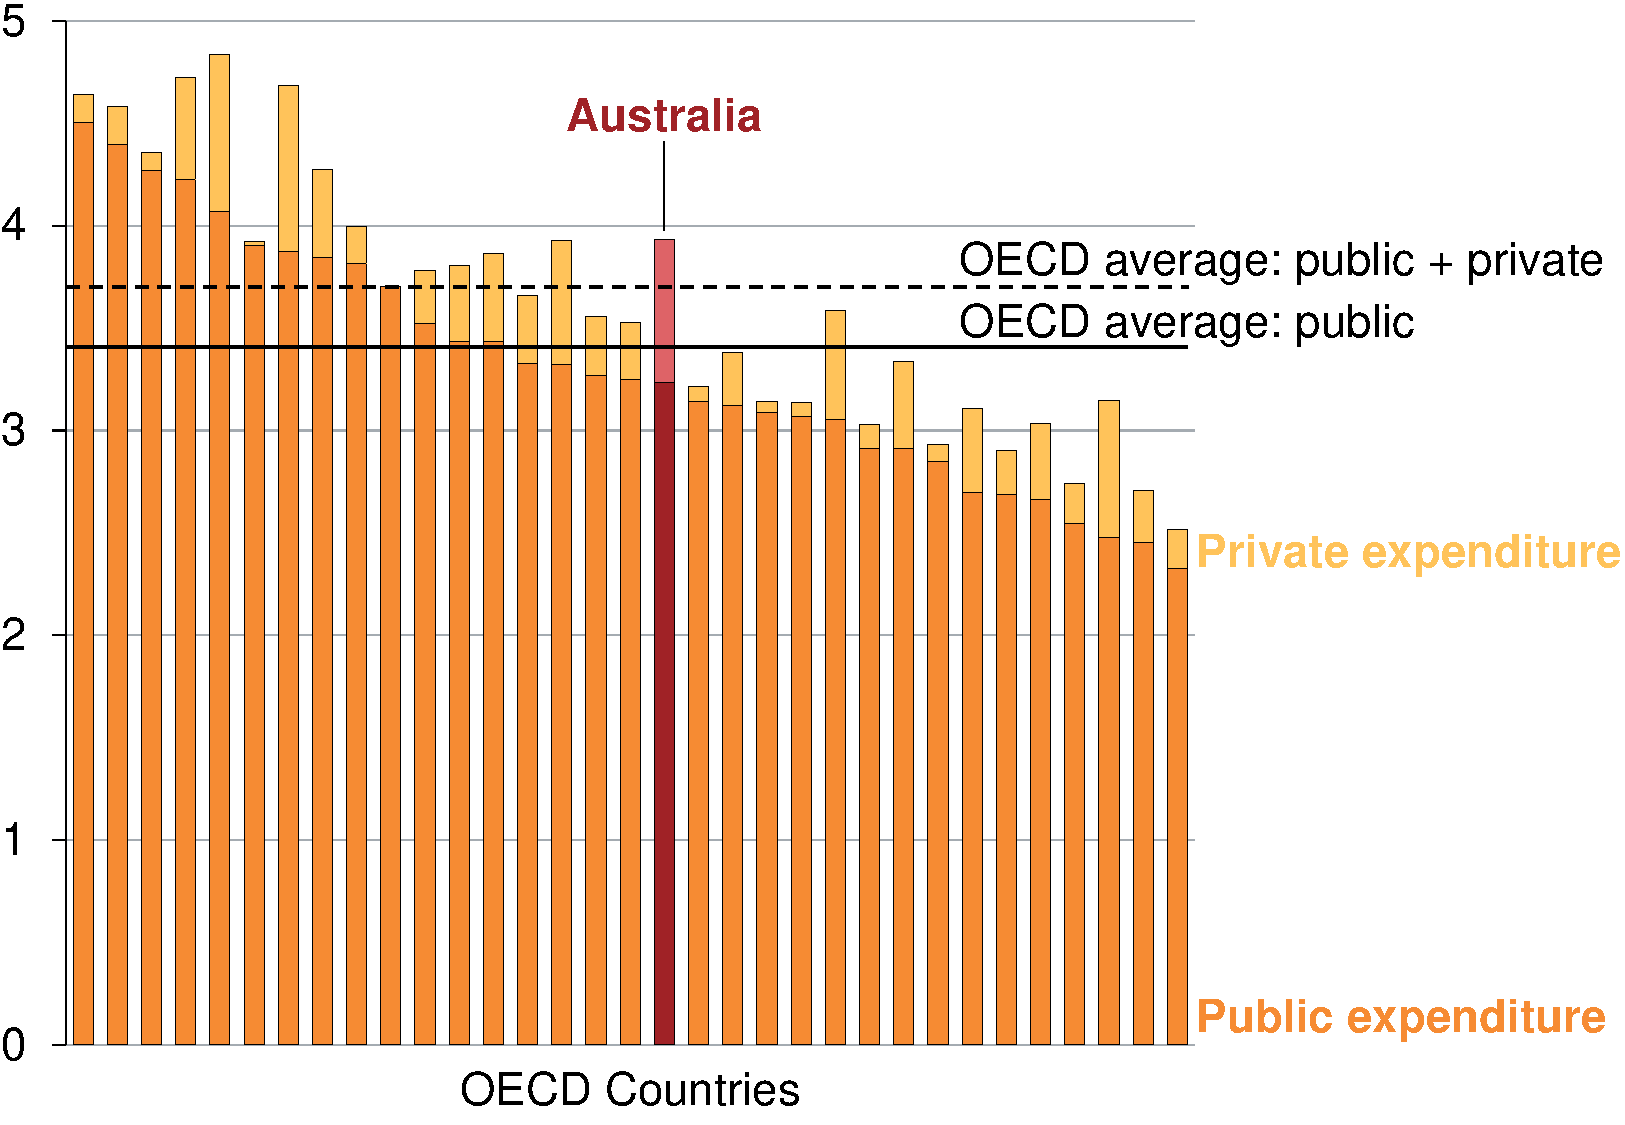
\includegraphics[page=1]{atlas/Charts.pdf}
\noteswithsource{Effect sizes represent the size of the difference between two groups – one group that receives an intervention and a similar group that does not. An effect size of 1 indicates an increase of 1 standard deviation in student achievement for the intervention group. The effect sizes shown here are average effects across multiple studies.}%
{\textcite{Hattie2008visiblelearningsynthesis}}
\end{figure}


\section{Learning, not silence, must be the end goal}\label{sec:learning-not-silence}
The teacher's ambition should not necessarily be a quiet classroom, but a genuinely productive class. \footcite{Watkins2013DisposedToLearn} The broader aims are to help students feel comfortable, be confident in their own abilities, be willing to participate and make mistakes, and be keen to challenge themselves in learning. 

\begin{figure}
\captionsetup{oneside, margin={0cm,-1em}}
\caption{Students disengage in a variety of ways\label{fig:students-disengage-variety-ways}}
\includegraphics[page=2]{atlas/Charts.pdf}
\noteswithsource{* Called uncooperative students in \textcite{Angus2009PipelineProject}. Serious behavioural issues, such as bullying or aggression, are out of scope for this report. Category size is indicative only, based on data from \textcite{Angus2009PipelineProject}}%
{Grattan framework, based in part on \textcites{Angus2009PipelineProject}{Sullivan2014PunishThemEngage}}
\end{figure}
 
And effective teaching goes further: creating an environment that not only makes learning possible now, but also teaches attitudes and behaviours that enhance learning and success in later life. Student skills in self-regulation, such as self-monitoring and self-evaluation, are vital for life-long learning.

What the teacher does, particularly in the early years of schooling, plays a big role in developing students' broader skills at school and work.%
    \footcites{Watkins2005ClassroomsLearningCommunities}{Watkins2013DisposedToLearn}
Explicitly teaching behaviours for learning is important, especially for those students who have not developed them at home. 

\section{There is a clear body of knowledge about what works best}\label{sec:clear-body-knowledge}
Major studies consistently identify a similar set of evidence-based approaches teachers should adopt to create effective classrooms.%
    \footcites{Hattie2008visiblelearningsynthesis}{Marzano2003ClassroomManagementWorks}{Simonsen2008EvidenceBasedPractices}
A mix of preventive and responsive approaches is needed.%
    \footnote{Other groupings exist, for example, Marzano's seven elements (\textcite{Marzano2003ClassroomManagementWorks}) and the National Council on Teacher Quality's ‘Big Five' (\textcite{Greenberg2014TrainingOurFuture}).}

Preventive approaches include setting high expectations for learning and behaviour, building strong relationships with students, and providing clear instructions. Responsive approaches include encouragement and praise, as well as consistent consequences and corrections. 

The challenge for teachers lies not only in knowing \emph{what} to do in theory, but learning \emph{how} to put that into practice. Any parent knows that the best intentions can disappear under pressure -- yet we expect teachers to get it right every day.

\section{Universal strategies can defuse minor problems early on }\label{sec:universal-strategies}

This report focuses on evidence-based techniques that can be applied to help engage all students in learning. Pro-actively establishing a positive classroom environment, and  understanding triggers for individual students, can help prevent minor behaviours escalating and becoming more serious down the track.%
    \footnote{\textcite{ShuklaMehtaAlbin2003TwelvePracticalStrategies}. Major empirical studies on student behaviour emphasise the importance of teachers pro-actively putting in place universal preventive strategies, with balanced responses, to improve student behaviour  and learning \textcites{Greenberg2014TrainingOurFuture}{Simonsen2008EvidenceBasedPractices}.}

Of course, in some situations, regardless of what the teacher does, some students may escalate behaviours, including verbal aggression and even physical violence. This report does not cover strategies for dealing with very serious behavioural issues or disorders. Nor does it examine strategies for students with disabilities, special learning needs, or serious mental health problems. These cases warrant specific approaches beyond the scope of this report.%
    \footnote{For more information on these topics, see \textcites{Friend2014IncludingStudentsSpecial}{Sutherland2008ExaminingInfluenceTeacher}{Walker1995AntisocialBehaviorSchool}.}
    %\footnote{\textcolor{red}{Cite literature on this -- need to search!!!}.} %!!! 
 

\chapter{Many students are disengaged in Australian classrooms }\label{chap:many-students-disengaged}
 
This chapter examines the learning climate in Australian classrooms. We draw on several major Australian academic studies over the past decade that provide in depth information on the situation in our classrooms.%
\footnote{Appendix~\topref{chap:appendix-a-australia-middle-pack} provides a brief overview of international comparisons on classroom climates and student engagement.}
 
The research paints a consistent picture of widespread low-level passive disengagement and disruption. It is not just about noise: a surprising number of students are quietly disengaged but otherwise compliant.
 
Little is known about why students are disengaged, although some data points to students being bored or finding work too difficult. We do know that classrooms characterised by disengagement are bad news, for the students and their teachers. Unproductive students perform much worse than their peers – and their behaviour impinges on the learning of others in the same class. 
 
The problem is widespread, but much worse in schools with many low socio-economic students. 

\section{Classrooms are not out of control but many students are not engaged in learning}\label{sec:not-out-of-control}

\begin{figure}
\caption{About 40 per cent of all students are regularly unproductive in a given year\label{fig:40-pc-regularly-unproductive}}%
\units{Percentage of students}
\includegraphics[page=3]{atlas/Charts.pdf}
\noteswithsource{* Called uncooperative students in \textcite{Angus2009PipelineProject}. Percentage of students productive vs. unproductive is averaged across 4 years (2005-2008).}%
{\textcite{Angus2009PipelineProject}}
\end{figure}

A major 2009 study in Western Australia that tracked 1,300 students found that about 40 per cent of students displayed unproductive behaviours regularly in a given year  (\Vref{fig:40-pc-regularly-unproductive}).%
    \footnote{\emph{The Pipeline Project} by \textcite{Angus2009PipelineProject}. The study had a  particular focus on low socio-economic schools.} 

Of the unproductive group, a surprisingly high number (over half) were compliant but disengaged – they were inattentive or lacked motivation. Only about one quarter of the unproductive students were disruptive, while the remaining quarter displayed non-compliant, erratic or aggressive behaviours.

\begin{figure}
\caption{Passive disengagement and disruption are common\label{fig:disengagement-disruption-common}}%
\units{Percentage of teachers who report behaviours occurring ‘almost daily', ‘daily' or ‘several times daily'}
\includegraphics[page=4]{atlas/Charts.pdf}
\source{\textcite{Sullivan2014PunishThemEngage}}
\end{figure}

In a 2014 study in South Australia, teachers similarly reported widespread problems with a lack of engagement.%
    \footnote{\emph{The Behaviour at School Study} 
    by \textcite{Sullivan2014PunishThemEngage}. The study surveyed 1,380 teachers in schools across South Australia .}
The study found that low-level disruption and disengagement occurred ‘almost daily or daily' in most classrooms  (\Vref{fig:disengagement-disruption-common}).
Common minor behavioural issues included talking out of turn, avoiding work, being late for class and being deliberately disruptive. Contrary to popular perception, aggressive and anti-social behaviours such as verbal abuse and physical violence were less common. %(\Vref{fig:disengagement-disruption-common}).

Of course, where they do occur, serious behaviours are difficult to manage. One study estimates that almost 10 per cent of Australian teachers work in schools where intimidation or verbal abuse of staff by students occurs weekly. This figure is much higher than in other countries surveyed (where the average was 3.4 per cent).%
    \footnote{\textcite{Freeman2014AustralianTeachersLearning}. This data is reported by the school principal.} 

\subsection{Disengagement is worse in low socioeconomic schools}\label{subsec:low-engagement-higher}

The 2014 South Australian study shows that low socioeconomic (SES) schools have higher rates of disengagement and low-level disruption. More than 60 per cent of teachers in low-SES schools report disruption in class several times daily, whereas only 10 per cent in high SES schools report such problems (see \Vref{fig:unproductive-behaviours-low-SES}).
    \footcite{Sullivan2014PunishThemEngage}

\begin{figure}
% Consider allowing this caption to protrude into the margin (for release)
\caption{More teachers report unproductive behaviours as very common in low-SES schools\label{fig:unproductive-behaviours-low-SES}}%
\units{Percentage of teachers who report behaviours ‘several times daily', by school socioeconomic status, selected behaviours}
\includegraphics[page=6]{atlas/Charts.pdf}
\noteswithsource{ICSEA is the Index of Community and Socio-Economic Advantage. A low score means a more disadvantaged school}{\textcite{Sullivan2014PunishThemEngage}}
\end{figure}

However, students from low-SES backgrounds do not inherently misbehave. Many disadvantaged schools have few behavioural problems.%
    \footnote{Some low-SES schools have much better than expected levels of engagement with schoolwork, see \textcite{Angus2009PipelineProject}.}
Higher rates of misbehaviour may reflect problems at home, or relate to the higher proportion of early career teachers in these schools.%
    \footcite{Freeman2014AustralianTeachersLearning} 
The uneven distribution of experienced teachers across the system can make the job harder for those in low-SES schools.

\section{Little is known about \emph{why} students are not engaging, but boredom is an issue}\label{sec:little-known-about-why}
Data on what drives passive disengagement and low-level disruption in Australian classrooms is limited. They could be consequences of students being uninterested in the curriculum, students being unhappy at home or in the schoolyard, or poor quality teaching.%
    \footnote{Students who are well behind or ahead of their classmates may find it difficult to engage with material unless it is tailored to the appropriate level of difficulty for them.
    This has been the subject of a previous Grattan Report: \textcite{Goss2015TargetedTeachingHow}.}
 
Some studies point to some students being bored while others find the work too hard. Two large international studies (one quantitative, one qualitative) evaluate students' reasons for misbehaving and not participating. The top reasons in the quantitative study were boredom, attention-seeking, and work-related difficulties (students didn't believe they could do it, so they didn't try). The qualitative study also identified boredom, as well as teacher-student misunderstandings and students' negative attitudes towards school.%
    \footnote{Reported in \textcite{Montuoro2015StudentPerceptionsMisbehaviour}.
    These findings are in keeping with an older 2001 Queensland School Reform Longitudinal Study which found that maths and science pedagogies and assessment tasks were not intellectually demanding enough to engage many students, see \textcite{Lingard2001QueenslandSchoolReformFinalReport}.} 
 
These findings are supported by the 2015 NSW \emph{Tell Them From Me} student engagement survey.%
    \footnote{NSW Department of Education, unpublished student feedback data, NSW government schools, 2015.}
Only 55 per cent of Year 9 students surveyed reported being challenged in maths classes. The highest performing students were even less likely to report being challenged.%
    \footnote{The student survey results similarly show that high performing students in Year 5 are less likely to be challenged. About 70 per cent of low-performing Year 5 students report being challenged at school, falling to under 50 per cent of the highest-performing students.} %REWORD !!!
 
These studies shed some light on why some students disengage, although better information is still needed on the root causes. But  regardless of why it's happening, unproductive behaviour holds back both students and their classmates.

\section{Students who are disengaged perform worse over time}\label{sec:students-not-engaged-perform-worse}
Studies show that students who behave poorly tend to learn less. Students who disrupt classrooms often receive less support and encouragement, and more criticism and punishment, from their teachers. As a consequence, they may learn less still.

\begin{figure}
% Consider allowing this caption to protrude into the margin
\captionsetup{oneside, margin={0cm,-1.6em}}
\caption{Students who are disruptive and disengaged tend to achieve less\label{fig:lower-scores-on-average}}%
\units{Mean reading test score}
\includegraphics[page=5]{atlas/Charts.pdf}
\noteswithsource{* Called uncooperative students in \textcite{Angus2009PipelineProject}. Test scores are from the Western Australian Literacy and Numeracy Assessment (WALNA), a state-wide annual testing program.}%
{\textcite{Angus2009PipelineProject}}
\end{figure}

In the Western Australian study that tracked students over four years, unproductive students were on average one to two years behind their peers in literacy and numeracy (see 
\Vref{fig:lower-scores-on-average}).%
    \footnote{\textcite{Angus2009PipelineProject}. This holds for reading and numeracy findings in this study.}


\subsection{Quiet disengagement should not go under the radar}\label{subsec:quiet-disengagement-under-radar}
The Western Australian study shows that compliant but quietly disengaged students do just as poorly, on average, as disruptive students (see \Vref{fig:lower-scores-on-average}). Nearly one in four students falls into this category.%
    \footcite{Angus2009PipelineProject}  

Students can passively disengage in various ways.%
    \footnote{\textcite{Galton1999ChangesPatternsTeacher}.
    The original study, led by Maurice Galton in 1976, comprised thousands of observations of 489 primary school children and 58 teachers in the UK over three years.
    Galton's follow-up study in 1996 found many of the same behaviour types.}
Some are `intermittent workers': they work when they believe they are being watched, but tend to move off-task when an opportunity arises. Then there are `easy riders': they work more slowly than other students, finding ways to extend routine tasks without attracting their teacher's attention. This is particularly problematic because it lowers their teachers' expectations.%
    \footcites{Angus2009PipelineProject}{Galton1999ChangesPatternsTeacher} 
Less commonly, disengaged student are `ghosts' -- those who go completely unnoticed by the teacher.

Each form of quiet disengagement challenges the teacher. But all forms reduce learning. 

\subsection{Disruptive behaviour affects the learning of others}\label{subsec:disruptive-behaviour-affects-learning-others}
How much a student learns is affected -- positively and negatively -- by their peers' behaviour.
Peer misbehaviour can disrupt the entire class. Good peer behaviour -- studying diligently for a test, for example -- can rub off on a misbehaving student.%
\footcites{Carrell2016LongRunEffectsDisruptive}{McVicar2013RightPeerRight} 


Student behaviour and teacher behaviour also influence each other. Students are not passive spectators in their classroom, so the teacher's response to one misbehaving student can `ripple' through the room.%
\footcite{Kounin1958RippleEffectDiscipline}
The teacher may be able to defuse the situation quickly, refocus the class and move on. Or they might get caught up in managing difficult students and quickly lose the respect and engagement of others.

Peer misbehaviour can disrupt the entire class, and the problem is compounded if there are a large number of disruptive students in the one class, see \Vref{box:concentration-disruptive-students}.

\vfill
\begin{smallbox}{A large number of disruptive students in the one class costs a lot of lesson time%
\footcite[][Table 6.7]{Freeman2014AustralianTeachersLearning}}{box:concentration-disruptive-students}
There appears to be a tipping point at which the level of disruptive behaviour starts to seriously reduce teaching time. In Australian classes with less than 10 per cent of students with behaviour problems, teachers spend about 10 per cent of class time keeping order. This is on par with the average rate across other countries. However, Australian teachers with more than 10 per cent of students misbehaving spend nearly a quarter of the lesson keeping order. This is much higher than other OECD countries. It is not clear why Australia does so much worse on this measure.
\end{smallbox}


\chapter{Teachers struggle with low-level disengagement and disruption }\label{chap:teachers-struggle}
Teachers get stressed when students don't engage in learning -- even when that manifests as quiet lack of interest. It can be draining to continually re-engage students when their attention is regularly lost. We don't know exactly why this is happening, but it is clear that classroom environments are not as good as they should be. 
 
Teachers nominate passive disengagement and low-level disruptive behaviour as a more difficult issue than aggressive or violent behaviour -- perhaps because low-level problems arise more often.
 
Teachers are calling for more support. Many feel they are not well prepared to respond to students not engaging or misbehaving in class. New teachers say this is their number one `professional learning need'. More experienced teachers also report being stressed. Teachers in poorer schools are the most stressed of all.
 
Excessive stress is bad for the teacher, of course, but it can also damage their students. Very stressed teachers can fall into bad habits: snapping at disengaged students and making aggressive or sarcastic comments to poorly behaved students. Everyone loses.
 
\section{Minor behaviour issues are a real concern for teachers}\label{sec:minor-behavioural-issues}
In the South Australian study by \textcite{Sullivan2014PunishThemEngage}, nearly one-in-three teachers reported being ‘extremely stressed' or ‘very stressed' by the challenges of engaging and re-engaging students in class.%\footcite{Sullivan2014PunishThemEngage} 

\begin{figure}
\caption{More teachers find passive disengagement and low-level disruptive behaviour the most difficult to manage\label{fig:behaviours-most-difficult-manage}}%
\units{Percentage of teachers who report behaviour as ‘most difficult to manage'}
\includegraphics[page=7]{atlas/Charts.pdf}%
\source{\textcite{Sullivan2014PunishThemEngage}}
\end{figure}

%  'see \Vref' -> '\Cref' as you had a triple hyphenation and a 
% bad final line. Cref not Vref because it's too close to page
% boundary -- HP
More teachers nominated disengagement and low-level disruptive behaviour, rather than aggressive or violent behaviour, as the most challenging to manage (\Cref{fig:behaviours-most-difficult-manage}).%
\footnote{\textcite{Sullivan2014PunishThemEngage}. This is not to dismiss the difficulty of handling more serious behaviours when they do arise, albeit less frequently.} These low-level behaviours include avoiding school work, disrupting the lesson and talking out of turn.
\pagebreak[2]  % preferred but not mandatory

While new teachers struggle with behavioural problems, experienced teachers struggle too. These problems do not simply disappear as a teacher gains more experience, and there are many unproductive students in the classrooms of experienced teachers, as \Vref{fig:all-teachers-experience-unproductive-behaviour} shows.%
    \footnote{Comparing \textcite{Sullivan2014PunishThemEngage} and \textcite{Freeman2014AustralianTeachersLearning}, shows that about one third of teachers who are stressed have more than five years' teaching experience.} 
One NSW trial found no relationship between years of teaching experience and teachers' classroom climate skills, or student engagement and student self-regulation in class.%
    \footcite{Gore2016TeachingExperienceRelative}

\section{Some teachers are more stressed than others}\label{sec:more-stressed-than-others}
Student behaviour is a prominent concern in teacher surveys.%
    \footcites{Buchanan2013TeacherRetentionAttrition}{Feltoe2013ComparingTeacherStress}{Richards2012TeacherStressCoping}{Stoughton2007HowWillI}
Teachers in low-SES schools are particularly stressed by student behaviour, as \Vref{fig:more-teachers-stressed-low-SES} shows.
Disengaged behaviours are reported more frequently in these schools.%
    \footnote{\textcite{Sullivan2014PunishThemEngage}. See also \Vref{subsec:low-engagement-higher}.}

\begin{figure}
\caption{Experienced teachers see a lot of unproductive student behaviour, inexperienced teachers see even more\label{fig:all-teachers-experience-unproductive-behaviour}}%
\units{Mean reported frequency}
\includegraphics[page=8]{atlas/Charts.pdf}
\source{\textcite{Sullivan2014PunishThemEngage}}%
\end{figure}

\citetrackerfalse 
\doublecolumnfigure{
    \caption{More teachers are stressed by unproductive behaviours in low-SES schools\label{fig:more-teachers-stressed-low-SES}}%
    \units{Percentage of teachers `extremely stressed’ or `very stressed’ because of the challenges related to managing student behaviour}
    \includegraphics[page=12]{atlas/Charts.pdf}%
    \noteswithsource{School socio-economic categories use ICSEA, the Index of Community and Socio-Economic Advantage. A low score means a more disadvantaged school}%
    {\textcite{Sullivan2014PunishThemEngage}}
}{
    \caption{Dealing with difficult student behaviour is a high priority for professional learning\label{fig:high-priority-professional-learning}}%
    \units{\null\newline Top 10 professional learning needs of secondary teachers}
    \includegraphics[page=9]{atlas/Charts.pdf}
    \noteswithsource{Categories reflect the AITSL Graduate Teacher Standards.}%
    {\textcite{McKenzie2014StaffAustraliasSchools}}
}

Lastly, casual and part-time teachers call for extra support in engaging and managing students.%
    \footcites{Buchanan2013TeacherRetentionAttrition}{TEMAG2016ActionNowClassroom}{Mayer2014LongitudinalTeacherEducation} 
Such teachers may not have the benefit of time or continuity in developing strong student relationships and in setting clear expectations and class routines.

\citetrackertrue

\section{Teachers want more support}\label{sec:teachers-want-support}

Dealing with misbehaviour is a concern for all teachers. It is the number one professional learning need among new teachers, and a priority area of need for more experienced teachers (see \Vref{fig:high-priority-professional-learning}).%
    \footnote{\mbox{\textcite{McKenzie2014StaffAustraliasSchools}. This finding holds for both primary and secondary teachers}.}  % no line break
Over a quarter of experienced teachers say they need further professional development on this issue.%
    \footcite{McKenzie2014StaffAustraliasSchools}

Issues begin with teachers' initial training. Many teachers and school leaders are unsatisfied with how trainees are trained to engage students and manage behaviour in the classroom. In the most recent \emph{Staff in Australia's Schools} survey, only half of teachers reported that their pre-service course was helpful in `managing classroom activities to keep students on task'. Only a third said their course helped in `dealing with difficult student behaviour'.%
    \footcite{McKenzie2014StaffAustraliasSchools} 
 
Principals also see a problem. They rate classroom management as the number one challenge for new teachers.%
    \footcite{Mayer2014LongitudinalTeacherEducation} 
Only a third of principals believe new teachers are well prepared for managing classrooms.%
    \footcite{AITSL2015InitialTeacherEducation}


\section{Stressed teachers can fall into a vicious cycle}\label{sec:stressed-teachers-vicious-cycle}
Highly stressed teachers are more likely to respond badly to students who are disengaged.%
    \footnote{A robust empirical study in 2000 found that stressed teachers with low self-confidence in classroom management are more prone to `depersonalisation' (a negative or excessively detached response to other people). The more emotionally exhausted teachers are, the poorer their performances will generally be, see \textcite{BrouwersTomic2000LongitudinalStudyTeacher}.} 
A poor response can make matters worse by prolonging the interruption and distracting other students, which in turn can stress the teacher.

Teachers can get caught in this damaging cycle, responding to students who are not focused on the task at hand, thereby unintentionally disrupting other students, and losing the momentum of the lesson. 
 
Too often, teachers may punish a misbehaving student -- by giving them a detention, or sending them to the principal -- without first considering whether their own behaviour might be contributing to the problem.
 
Recognising the impact of negative responses under stress is not about blaming teachers. Some teachers face challenging classrooms and have ample reason to feel under pressure. As seen earlier, almost one in ten teachers work in schools where students intimidate or verbally abuse staff at least once per week.%
    \footnote{\textcite{Freeman2014AustralianTeachersLearning}, as mentioned in \Vref{sec:not-out-of-control}.}
But the way those and other teachers respond makes a real difference.
\subsection{Some teacher responses are not as good as they could be}\label{subsec:some-teacher-responses}

\begin{figure}
\caption{Australian teachers' responses to student behaviour are far more negative than positive}\label{fig:responses-more-negative}
\units{Percentage of teacher responses to students }
\includegraphics[page=10]{atlas/Charts.pdf}
\noteswithsource{Responses have been standardised}%
{Study 1: \textcite{CluniesRoss-2008-Use-proactive-reactive-classroom-mgmt} survey of 97 primary teachers from Melbourne. Study 2: Wheldall and Beaman (1994) observation of 36 primary teachers from seven Sydney schools. Study 3: Wheldall and Beaman (1994) observation of 79 secondary teachers from four Sydney schools, reported in \textcite{BeamanWheldall-2000-Teachers-use-of-approval-disapproval}.}
\end{figure}

%!!! FIND REFS (Julie - can the original studies be cited in this source for this figure?)

Several studies show that Australian teachers could respond better to disengaged behaviours in the classroom.%
    \footcites{Lewis2008StudentsReactionClassroom}{Montuoro2015StudentPerceptionsMisbehaviour}
For instance, teachers tend to reserve praise for good work rather than good behaviour (see \Vref{fig:responses-more-negative}).
This may suggest teachers see good behaviours as a given, not requiring recognition or reinforcement.
 
The balance of positive and negative interactions will be different for every teacher-student relationship. But students who interact mainly negatively with their teacher are likely to develop bad attitudes in class (and of course the two are reinforcing).
 
Teacher-student misunderstandings may arise because what teachers believe they should do and what they actually do are not always in sync.%
    \footcite{Fang1996ReviewResearchTeacher}
Teachers believe they should warn and give explanations to students they punish. But they often do not do so in practice. An Australian survey of students who had been sent out of the classroom showed that only 30 per cent believed they had been given a warning before they were excluded. Only 40 per cent reported that the teacher gave them a reason for their removal.%
    \footcite{Lewis2012ExcludingStudentsClassroom}
And teacher and student had a follow-up conversation in fewer than half of the incidents.%
    \footnote{\textcite{Lewis2012ExcludingStudentsClassroom}. Those students who did receive an explanation were significantly more likely to accept responsibility and less likely to blame the teacher.}

\subsection{Some teachers still get aggressive in their classroom}\label{subsec:some-teachers-get-aggressive}
Aggressive behaviour by teachers -- including punishing entire classes, yelling, humiliating students or being sarcastic towards students -- distracts students and impedes academic and social-emotional learning.%
    \footcites{Lewis2008StudentsReactionClassroom}{Lewis2001ClassroomDisciplineStudent}{RileyBrew2010WhyDidYouDoThat} 
 
Despite this, teacher aggression towards students still occurs in many Australian schools, albeit infrequently. A 2005 study of teachers' classroom management strategies, drawing on the views of more than 4,000 students and nearly 500 teachers, reported that some teachers were aggressive ‘some of the time'. The study found that such aggressive behaviours distracted students and made them feel worse towards their teacher.%
    \footcite{Lewis2008StudentsReactionClassroom}  

In a more recent survey of almost 500 Victorian teachers, most reported using aggressive strategies `hardly ever' or `never'. But a third conceded they had yelled angrily at students, at least sometimes. And almost half reported making sarcastic comments to students who misbehave, sometimes or most of the time.%
    \footcite{Romi2011ImpactTeachersAggressive}
 
A common theme is that teacher aggression emerges when the teacher is stressed and tired: \emph{``I don't mean to -- they just happen''}.%
    \footcite{RileyBrew2010WhyDidYouDoThat}
Stressed teachers need support but may be the least likely to ask for help.%
    \footcite{Lewis2001ClassroomDisciplineStudent} 
 
Poor-performing teachers tend to express the belief that factors totally outside their control `determine' student outcomes.%
    \footcite{Lingard2001QueenslandSchoolReformFinalReport}

Teaching practice cannot improve without teachers accepting some responsibility and seizing opportunities to improve.
But there's no doubt it's hard.
 
\section{A no-lose part of the solution is creating better classroom environments}\label{sec:no-lose-part-of-solution}
As discussed in \Chapref{chap:many-students-disengaged}, there is little data on exactly why students are disengaged in Australia. The problem won't be fully solved until we get a better understanding of its root causes of disengagement. Other factors, such as the quality of teaching, the curriculum, or problems at home could be at play.
 
But we can and should get to work immediately on one important part of the solution: building the capacity of teachers to create classrooms that improve learning. 
 
If we do nothing, the problem is likely to only get worse: teacher stress and job dissatisfaction will fester, and minor problems in class will be mishandled and so escalate to more serious flare-ups. 

\chapter{How to create classrooms that improve learning}\label{chap:what-works-best}

There is a clear body of knowledge of what works best to create an effective learning environment. This chapter examines what approaches and techniques work well, \emph{and} how teachers can apply them in practice. A key challenge for teachers is knowing not only what to do, but learning how and when to do it.
 
\emph{Part A: `What works best'} gives a synthesis of the research. A mix of preventive and reactive strategies are best, along with a balance of approval and disapproval of student behaviours. 
 
\emph{Part B: `How to implement what works best'} shows the steps that can help turn theory into practice, drawing on a recent US synthesis of the evidence. Teachers will be most effective if they know their students well and understand the triggers for different student behaviours. Given this skill set is highly nuanced, teachers need opportunities to develop their strategies in classroom settings, assisted by feedback from their colleagues.

\addindentchap{Part~A: What works best}\label{sec:part-a-what-works}

Several big studies highlight specific evidence-based techniques for creating an effective learning environment.%
    \footnote{Key meta-studies used in this chapter include: \textcites{Greenberg2014TrainingOurFuture}{Hattie2008visiblelearningsynthesis}{Marzano2003ClassroomManagementWorks}{Simonsen2008EvidenceBasedPractices}.}
As always, prevention is better than cure. Teachers need to be able to quickly and accurately identify student behaviour that might become a problem (this attribute is sometimes called ‘with-it-ness').%
    \footcite{Marzano2003ClassroomManagementWorks}
But the classroom teacher cannot rely solely on preventive strategies; effective \emph{responses} and \emph{reactions} are also necessary.

\citetrackerfalse

In this chapter we synthesise the common approaches highlighted in the research. They are:%
    \footnote{Other groupings exist, for example, Marzano's seven elements (see \textcite{Marzano2003ClassroomManagementWorks}) and the National Council on Teacher Quality's ‘Big Five' (see \textcite{Greenberg2014TrainingOurFuture}).}
    
\citetrackertrue

\begin{tabularx}{\columnwidth}{>{\normalsize}p{7.5cm}*1{>{\arraybackslash\normalsize}X}}
\begin{tabular}{>{\normalsize}p{7.5cm}}{\normalsize} 
\tabitem High expectations \\
\tabitem Strong teacher-student relationships \\
\tabitem Clarity and structure in instruction  \\
\tabitem Active learning \\ \end{tabular} 
&   \(\begin{array}{l} \MyLBrace{7.5ex}{Preventive} \end{array}\) \\
\begin{tabular}{>{\normalsize}p{7.5cm}} \tabitem Encouragement and praise \\ \tabitem Consistent corrections and consequences \\ \end{tabular}
&   \(\begin{array}{l} \MyLBrace{3.75ex}{Responsive} \end{array}\)
\end{tabularx}

\section{Preventive approaches}\label{sec:preventive-approaches}
Preventive approaches attempt to avoid behaviour problems by focussing students' attention on their learning.

\subsection{High expectations for every student}\label{subsec:high-expectations-every-student}
Effective teachers instil in every student an expectation of success. They recognise that student motivation, engagement and self-belief can drive student achievement -- and vice versa.%
    \footcite{OECD2013PISA2012ResultsReadyToLearn}  
 
When students achieve success, their self-esteem lifts and they become more engaged, which leads to even better performance. Competence breeds self-esteem and confidence, which in turn breeds greater competence.%
    \footcites{Brophy2013MotivatingStudentsLearn}{Porter2007StudentBehaviourTheory}
 
Student expectations of their own performance draw on their prior achievements.%
    \footcite{Hattie2008visiblelearningsynthesis} 
In some cases, these expectations could be limiting, and a circuit-breaker is required.%
    \footcite{Hattie2008visiblelearningsynthesis}
The expectations of a child are ``powerful enhancers of -- or inhibitors to -- school education''.%
    \footcite[][31]{Hattie2008visiblelearningsynthesis}

Teachers' bias in expectations can also be self-fulfilling for the child or young person. For example, high expectations for a student could translate into the student putting in more effort and the school devoting more resources to that student. The reverse can also be true: low expectations can translate into less effort and fewer resources.%
    \footnote{Recent work by the US Institute of Labour Economics shows that teacher expectations have a causal impact on achievement, see \textcite{PapageorgeGershenson2016TeacherExpectationsMatter}.}

One strategy teachers can use to raise a student's expectation of success is to recognise the student's early achievements and strengths.

\subsection{Good teacher-student relationships}\label{subsec:teacher-student-relationships}
Students who have a good relationship with their teacher tend to succeed at school.%
    \footcites{Hattie2008visiblelearningsynthesis}{Marzano2003ClassroomManagementWorks}
This is particularly the case for younger students. It can be the difference between a student accepting or resisting classroom rules that enable learning.%
    \footcite{Marzano2003ClassroomManagementWorks}
Teachers with good relationships with their students can more effectively intervene when problems arise.%
\footcites{Epstein2008ReducingBehaviorProblems}{Marzano2003ClassroomManagementWorks}{Montuoro2015StudentPerceptionsMisbehaviour}

\begin{verysmallbox}[t]{Explicit modelling of learning behaviours%
\footcites{Brophy2006HistoryResearchClassroom}{Watkins2005ClassroomsLearningCommunities}}{box:explicit-modelling-learning-behaviours}
Teachers often assume students have the skills to behave, or that they know how to be disciplined but choose not to be. This is not necessarily the case. The skills of self-discipline and sustained application to work need to be taught and continually reinforced in the early years of school. Teachers may also need to teach social and emotional language so that students can understand others and to appropriately express themselves.
 
Teachers should identify those behaviours in which students need explicit instruction, and teach those skills by providing examples, opportunities for practice, and positive reinforcement when students behave appropriately. 
\end{verysmallbox} 

It is not about whether students `like' their teachers. The studies show that the best teacher-student relationships form when the teacher gives strong guidance, and shows clear purpose as well as concern for the needs of others and a desire to work as a team.%
    \footcite{Marzano2003ClassroomManagementWorks} 
Mutual respect is important; teachers should recognise students' rights to learn, to feel emotionally and physically safe, and to be treated fairly.%
    \footcites{Lewis2011DevelopmentalManagementApproach}{Rogers2015ClassroomBehaviourPractical} Empathy is vital, but strong relationships also require teachers to maintain `a healthy emotional objectivity' towards their students.%
    \footnote{\textcites{Hattie2008visiblelearningsynthesis}{Marzano2003ClassroomManagementWorks}. If teachers personalise student misbehaviour it can drive inappropriate teacher responses (for example teacher aggression) see \textcite{RileyBrew2010WhyDidYouDoThat}.}

Student-to-student relationships in the classroom matter too. Peers can positively influence each others' learning, through helping, tutoring, providing friendship, giving feedback, and making class a place students want to come to each day.%
    \footcite{Wilkinson-Fung-2002-Small-group-composition-peer-effects}
Teachers can encourage positive student-to-student relationships in various ways, for example through the use of group work and student feedback, as well as setting expectations for positive interactions with others in class.

\subsection{Clarity and structure}\label{subsec:clarity-and-structure}
Teachers must be clear and consistent about what students are expected to do, as well as teaching them how to do it.%
    \footcites{Marzano2003ClassroomManagementWorks}{Simonsen2008EvidenceBasedPractices} 
Studies show teacher clarity is a key to student achievement (see \Vref{fig:classroom-environment-factors}).%
    \footcite{Hattie2008visiblelearningsynthesis}

Students respond well to rules and routines for classroom activities. Teachers need to teach students how to perform the roles expected of them, and the best teachers become role-models of the behaviours required (see \Vref{box:explicit-modelling-learning-behaviours}).\footcite{Brophy2006HistoryResearchClassroom}

Teachers should also explicitly state the learning goals, define and explain classroom procedures, direct activities, and minimise distractions.\footcites{Greenberg2014TrainingOurFuture}{Marzano2003ClassroomManagementWorks}{Simonsen2008EvidenceBasedPractices}

\subsection{Active learning}\label{subsec:active-learning}
Student participation is a critical part of effective teaching and learning. Without opportunities to speak, problem-solve and work with others, students may quietly disengage or become restless -- and teachers may not know if those students are learning. 

\begin{verysmallbox}[!t]{Methods for monitoring student engagement in learning and eliciting feedback}{box:monitoring-student-engagement}

\textbf{Response cards:} The teacher asks a question of the class. Each student writes their answer and holds it up. The teacher can then scan the room to see who is following and who may need help. 

\textbf{‘No hands up':} The teacher puts the names of all the students in a hat. The teacher asks a question, and draws a name from the hat. The student whose name is drawn answers the question. This sets an expectation that all students should be ready to respond at any time during the lesson.

\textbf{Exit cards:} At the end of a lesson, the teacher asks their students to write down their main take-away from the lesson (or a question arising from the lesson). The students give their answer to the teacher on their way out. Exit cards help the student to consolidate their learning and enable the teacher to monitor each student's understanding. Responding to students' exit card questions or reflections can also provide a good hook for the teacher to begin the next lesson.%
\footnote{See \textcite{Simonsen2008EvidenceBasedPractices} on the value of response tools.}

\end{verysmallbox}

\citetrackerfalse

The more opportunities students have to respond in class, the more likely they are to learn well.%
    \footcite{Simonsen2008EvidenceBasedPractices} 
Two specific ways teachers can provide regular opportunities for students to respond are through use of response cards, on which every student can write and hold up their answer, and guided notes, which highlight the main ideas of a lesson, with space for students to expand on them. (See \Vref{box:monitoring-student-engagement}).
 
Opportunities to collaborate with peers and do group work also improve a student's achievement, interpersonal relationships and attitudes to learning.%
    \footcite{Marzano2003ClassroomManagementWorks}
 
Class-wide peer tutoring programs (where one student coaches another) can also increase academic engagement and reading achievement.%
    \footcite{Simonsen2008EvidenceBasedPractices}
 
\citetrackertrue

\section{Responsive approaches}\label{sec:responsive-approaches}
A typical class will have both behaviours the teacher should encourage and those the teacher should discourage. How the teacher responds is critical to whether problems are resolved quickly or fester and become larger. 
The teacher's responses should include a combination of approval and disapproval. One large study found that positive reinforcement was on average more effective than punishment, but that a combination of the two was most effective of all.%
    \footnote{\textcite{Stage1997MetaanalysisInterventionsDecrease} reported in \textcite{Marzano2003ClassroomManagementWorks}.}

\subsection{Encouragement and praise}\label{subsec:encouragement-and-praise}

\begin{verysmallbox}{The right and wrong kinds of praise%
    \footcites{Epstein2008ReducingBehaviorProblems}{Greenberg2014TrainingOurFuture}}{box:right-and-wrong-praise}

\textbf{Do \dots}
 
 \begin{itemize}
    \item be specific about the behaviour you are praising
    \item give praise immediately after the appropriate behaviour
    \item praise the process or action
\end{itemize}

\textbf{Don't \dots}
\begin{itemize}
    \item praise the person or trait (\eg, ``Jill is such a good girl'')
    \item use reinforcers for a task that students already want to do
\end{itemize}

\end{verysmallbox}

Positive reinforcements include praise, encouragement and rewards. Praise should be specific and genuine.%
    \footcite{Simonsen2008EvidenceBasedPractices}
If it is vague or overdone it can come across as insincere, can lower expectations, and can undermine the authenticity of the teacher's relationship with the student (see \Vref{box:right-and-wrong-praise}).

Positive attention and genuine encouragements such as ``good job'' are also valuable. A popular encouragement, known as `catching students being good', uses a note, cue or quiet word to subtly recognise and reinforce appropriate learning behaviours.%
    \footcite{Marzano2005HandbookClassroomManagement}
 
Giving rewards, such as tokens for privileges, can be effective. They are most effective when both given for positive behaviour and removed for negative behaviour.%
    \footcite{Marzano2003ClassroomManagementWorks}
But giving rewards can undermine student responsibility, and so should only be done in concert with other approaches.%
    \footcite{Bear2015PreventiveClassroomBased}
 
\subsection{Corrections and consequences}\label{subsec:corrections-and-consequences}
Consequences have a place in the classroom, just as they do in life. Students are unlikely to maintain good behaviour in the absence of consequences, and teachers need options when things get out of control.%
    \footcite{LewisMontuoro2013SelfPredictedClassroom}   
 
But it is not appropriate for teachers to always jump straight to punishment without some warning, a `correction', which gives the student an opportunity to change their behaviour. 
 
Corrections can reduce the prospect of behaviour getting worse and requiring punishment. Scanning the class for students disengaged and then acting quickly – moving closer to a student, making eye contact, or pausing – can make a student aware of their behaviour and allow them to adjust it themselves.%
    \footcites{Lewis2011DevelopmentalManagementApproach}{Rogers2015ClassroomBehaviourPractical} 
Verbal corrections, such as a warning, should be brief, calm and clear about what is required.%
    \footcite{Simonsen2008EvidenceBasedPractices}

If punishments are necessary they should always have a clear learning purpose. The teacher must explain to the student why they are being punished and, in particular, highlight how the misbehaviour affects the student’s own learning and/or the learning of others.%
    \footcites{Lewis2011DevelopmentalManagementApproach}{Rogers2015ClassroomBehaviourPractical}

Teachers often confront the balancing act of how much attention to give a misbehaving student. Teacher attention is an incentive for many students, so `tactical ignoring’ of minor issues, in combination with praise for appropriate behaviour, can encourage better behaviour.%
    \footcite{Simonsen2008EvidenceBasedPractices}

 \begin{smallbox}{Exclusionary practices should be a last resort}{box:exclusionary-practices-last-resort}
Schools and teachers sometimes resort to exclusionary practices -- such as time-outs, streaming students into special classes or suspensions -- to address more serious behavioural issues. 
 
Time-outs have been shown to work well under certain conditions, for example when students are removed from a reinforcing environment (such as socialising with peers) and placed in a non-reinforcing environment (such as an isolated desk) for short periods.%
    \footnote{\textcites[][365--6]{Sullivan2014PunishThemEngage}[][141]{TurnerWatson1999ConsultantsGuideTimeOut}. Students respond better when they are made aware of how their actions lead to the need for a time-out, see \textcite[][139]{TurnerWatson1999ConsultantsGuideTimeOut}.}
But time-outs can easily backfire. Sending a student away from the class may reinforce negative behaviours if they are acting up to avoid school work.%
    \footcites{InterventionCentralNDTimeOutReinforcement}{TurnerWatson1999ConsultantsGuideTimeOut} 
They can also damage teacher-student relationships, as well as the individual's learning.%
    \footcites{InterventionCentralNDTimeOutReinforcement}{TurnerWatson1999ConsultantsGuideTimeOut}{Wilhoit2000GuidelinesEffectiveUse}
 
Streaming disruptive students into special classes and suspensions can reduce the learning of those students.%
    \footcites{Graham2016CaughtBetweenRock}{Muller2010NegativePeerInfluence}{Skiba2008SafteyWithoutSuspensions} 
Suspensions are one of the most serious forms of punishments, but it is unclear if they help to rehabilitate students, especially if the home environment is not conducive to reflection.%
    \footcites{Kohistani2015SchoolSuspensionBeneficial}{Osher2010HowCanWeImprove}
\end{smallbox}

This report does not analyse how teachers and schools should best handle more serious behavioural problems. However, \Vref{box:exclusionary-practices-last-resort} gives a brief overview of what the evidence tells about extended time-outs, suspensions and expulsions. One thing is clear: these exclusionary practices can sacrifice one student’s opportunity to learn in order to improve the learning environment for the rest of the class or school. This trade-off raises ethical questions and such practices should be used as a last resort.
\clearpage
\addindentchap{Part~B: How to implement what works best}\label{sec:part-b-how-to-implement}
\vspace*{0.5\baselineskip}
Teachers need to be aware of the evidence about strategies to improve the learning environment. But they need to know not only \emph{what} to do, but to learn \emph{when} and \emph{how} to do it.%
    \footnote{Various models and guides exist that can help teachers to better employ evidence-based strategies in their classrooms. Guides include: \textcites{Epstein2008ReducingBehaviorProblems}{Greenberg2014TrainingOurFuture}{Marzano2003ClassroomManagementWorks}. Models include: \textcites{Alberto2012AppliedBehaviorAnalysis}{Evertson1995ClassroomOrganizationManagement}{PBIS2017PositiveBehavioralInterventionsSupports}{Rogers2015ClassroomBehaviourPractical}. See \textcites{EvertsonWeinstein2013HandbookClassroomManagement}{ONeillStephenson2014EvidenceBasedClassroom} for model comparison.}
The process involved in testing different strategies and assessing what works best for different students is not an easy one.
\section{The four key steps}\label{sec:four-key-steps}

\begin{figure}
\caption{The process for learning how to use evidence-based techniques\label{fig:what-teachers-can-do}}
\includegraphics[page=11]{atlas/Charts.pdf}
\source{Adapted from \textcite{Epstein2008ReducingBehaviorProblems}.}
\end{figure}

The US `What Works Clearinghouse’ provides a process guide for teachers in how to reduce behaviour problems in the classroom (\Vref{fig:what-teachers-can-do}).%
    \footcite{Epstein2008ReducingBehaviorProblems}
This guide involves an `adaptive teaching’ approach, where teachers first analyse student behaviours, trial different approaches, then adopt what works best. We use this synthesis to identify four key steps teachers can take.

The first step is that teachers must know their students and the specifics of any behaviour issues, including passive disengagement. Teachers need to be able to identify the conditions that prompt and reinforce behaviours, so that they can tailor effective and efficient responses. A key issue is considering how the teacher's own behaviour might be contributing to the problem. This is critical. 
 
Second, teachers should proactively manage the classroom environment, altering or removing factors that trigger problem behaviour. They should revisit and reinforce expectations of student behaviour and learning in the classroom. If needed, teachers should rearrange the classroom schedule or learning activities to better meet students’ needs, or adapt instruction to individual students to promote their engagement.
 
Third, teachers should model and reinforce good behaviour. Teaching and reinforcing new skills can increase appropriate behaviour and enhance a positive classroom climate. This includes teaching students socially- and behaviourally-appropriate skills, to replace problem behaviours. Teachers can help students to know how, when, and where to use these new skills.

Fourth, teachers should collaborate with colleagues and experts to discuss issues and potential solutions. Taking opportunities to observe teachers who have created successful classrooms is important, for example seeing how something is said to a particular student, or how the behaviour of another student is tactically ignored (see \Vref{box:collaboration-with-colleagues}).
 
Of course, teachers can’t do this all on their own. The role schools should play is the subject of the next chapter.






\chapter{Schools can do more to empower teachers}\label{chap:schools-can-do-more}
Students, and indeed teachers, can get confused when there are different expectations for classroom behaviour and learning in each class. A consistent approach across the school is vital. 

Most school leaders already set consistent expectations. But they need to do more than that. They must ensure that teachers have the skills and tools to engage students in class. This includes providing intensive induction programs for new teachers, and regular opportunities for all teachers to observe their colleagues in the classroom and to receive and give feedback. Teachers need tools to be able to accurately assess and appropriately respond to the different behaviours of their students. And they need to have confidence that help is at hand from school leaders -- particularly for serious cases and sustained issues. 

\section{School-wide approaches are critical}\label{sec:consistent-school-wide-approaches}
Teachers are more likely to create effective classrooms when their school supports a common approach.%
    \footcite{Epstein2008ReducingBehaviorProblems}
Each school should have common expectations, a common language and a common understanding of appropriate behaviour for learning in class.

Many Australian schools already have a school-wide student behaviour plan.%
    \footnote{For example, the School-Wide Positive Behaviour Support model, also known as Positive Behaviour for Learning (PBL), is promoted in most states. And there are other less prescriptive approaches too, such as Ecological and Social-Emotional Learning approaches. Few of these models have been formally evaluated. See \textcite{ONeillStephenson2014EvidenceBasedClassroom} for more information.}
Typically, these articulate the school’s philosophy and values. Most ensure the school monitors student attendance and instances of bullying and other disciplinary issues. All schools should have such a plan. They are important in laying the ground rules and establishing consistency across the school.


There is increasing interest in positive psychology as an approach in many Australian schools, although evidence is still emerging on its effectiveness (see \Vref{box:role-positive-education}). This report does not examine which school-wide behaviour models work best, but focuses on the processes and structures that enable the chosen model to be implemented effectively. 

\section{Schools should also provide more practical support}\label{sec:school-behaviour-plans}
A school-wide behaviour plan is a key first step. But without intensive teacher training, little is likely to change in the classroom. 
 
Teachers need the time to step back: to identify the different student behaviours, identify triggers, analyse their own approaches, and to think about what preventive measures might work better. 
 
This is a complex and nuanced task. Opportunities to learn from experts, observation and collaboration can help teachers develop their skills, and can save time and energy down the track. 
 
This section outlines four practical things school leaders can do to help all teachers, especially new teachers, to build their classroom capabilities:
 
\begin{itemize}
    \item Better induction programs
    \item Opportunities to collaborate
    \item Tools to help teachers adapt their approaches
    \item Extra support for escalating issues
\end{itemize}

\subsection{Create better induction programs}\label{subsubsec:create-better-induction-programs}
The first couple of years in the classroom can be stressful and overwhelming for new teachers. The learning curve is steep: How can I keep the class focussed on the task at hand? How should I respond to students who are bored, or talk back, or play up?

New teachers need comprehensive induction programs to help them develop their practical skills and strategies. While many government guidelines actively promote the importance of induction programs, many Australian schools do not provide them.%
  \footnote{New AITSL national guidelines in 2016 put more emphasis on high-quality induction programs.} 
Only half of Australian teachers say they participated in an induction program as a new teacher.%
    \footcite[][Table 4.1]{OECD2014TALIS2013ResultsTeachingLearning}
    
Further, only about a third of early-career teachers have a mentor.%
   \footcite[][Table 4.4]{OECD2014TALIS2013ResultsTeachingLearning}
Without a mentor, young teachers will have fewer opportunities to learn from their more experienced colleagues and to see effective classroom techniques in action. 
 
High-performing schools systems do it better. In Shanghai, for example, every new teacher has two mentors, one for teaching and the other for classroom management.%
    \footnote{For further information see a previous Grattan report: \textcite{Jensen-2012-Catching-up-learning-from-best-in-East-Asia}.}

All Australian schools should have induction and mentoring programs that help new teachers with the difficult transition to the classrooms. And their mentors should be expert teachers who have shown the ability to pass on their knowledge of what works best in the classroom.

\begin{smallbox}{A role for positive psychology?}{box:role-positive-education}

Many schools embrace the philosophy of `positive psychology’ in education -- based on the idea that we learn more when we feel good. The aim is to build student resilience, well-being and achievement. An increasing number of schools practise this `positive education’.%
    \footnote{Many use Seligman’s PERMA model (positive emotions, engagement, relationships, meaning and accomplishment), see \textcite{Waters2011ReviewSchoolBased} and \textcite{Seligman2011FlourishVisionaryNew}.}

There is some evidence that positive psychology interventions can improve student performance, well-being and engagement.%
    \footcites{Durlak2011ImpactEnhancingStudents}{Waters2011ReviewSchoolBased} Some programs aim to build character strengths such as self-discipline. There is some empirical basis for this approach: for example, a longitudinal study of eighth-graders showed that self-discipline can be a better indicator than IQ of a student’s academic performance.%
    \footnote{\textcite{DuckSeligman2005SelfDisciolineOutdoes}, reported in \textcite{Waters2011ReviewSchoolBased}.}
 

Given some of the good early signs, positive education is a trend to watch. However, even advocates recognise that more reliable measures are needed before positive psychology can be taken more seriously in education policy.%
    \footcite{White2016WhyWontItStick}
\end{smallbox}

\CenturyFootnote

\subsection{Ensure teachers collaborate with colleagues}\label{subsubsec:ensure-teachers-collaborate}
Teachers are calling out for more support on how to keep students engaged. When asked how they could improve their skills in this area, teachers nominate collaboration with colleagues as their top suggestion.%
    \footcite{Sullivan2014PunishThemEngage}
%note that we say "crying out" in the media release!!!
Collaboration is especially important for developing this nuanced aspect of effective teaching (\Vref{box:collaboration-with-colleagues}). Working together with peers and experts on how to handle difficult situations is vital for teacher development.%
    \footnote{\textcites{Epstein2008ReducingBehaviorProblems}{Hough2011CharacteristicsEffectiveProfessional}. More broadly, teachers in schools with strong, trusting collegiate relationships among staff are more willing to learn and engage in new practices, see \textcite{Epstein2008ReducingBehaviorProblems}.}

Despite this, there are still too few opportunities for teachers to observe each other and collaborate on these skills and techniques (and effective teaching more broadly). Australian teachers tend to work behind closed classroom doors; too many are left on their own to try to figure out how to teach effectively.

Australia is well below the OECD average in terms of the proportion of teachers giving and receiving feedback generally.%
    \footcite[][359, 394]{OECD2014TALIS2013ResultsTeachingLearning}
More than 40 per cent of Australian teachers say they have never observed or given feedback to their colleagues.%
    \footcite[][128]{Freeman2014AustralianTeachersLearning}

\begin{smallbox}{Collaboration is especially important for developing nuanced skills to engage and manage students}{box:collaboration-with-colleagues}
\deffootnote{1.5em}{1.5em}{\makebox[1.5em][l]{\thefootnotemark.\ }}
While opportunities to collaborate, observe and receive feedback are important for developing any aspect of effective teaching, they are especially critical for creating positive classrooms and engaging students.%
    \footcites{Epstein2008ReducingBehaviorProblems}{Hough2011CharacteristicsEffectiveProfessional} 
 
A study of more than 2,300 teachers in 241 schools in the US found that professional learning about classroom behaviour was most effective when it was classroom-based, school-wide, and sustained over an extended period. Coaching from experts also greatly enhanced teaching and learning outcomes.%
    \footcites{Hough2011CharacteristicsEffectiveProfessional}
 
Engaging each student socially, emotionally and intellectually in learning requires a complex set of skills. It is hard work. It involves a lot of practical on-the-job judgement. Opportunities to observe how effective teachers approach situations, and to discuss problems in depth, are vital to helping teachers improve.
\end{smallbox}
% Silent CenturyFootnote:
\deffootnote{2.4em}{1.9em}{\makebox[2.4em][r]{\thefootnotemark.\ \ }}%

\subsection{Provide teachers with the tools to assess and improve their approaches to engaging students}\label{subsubsec:provide-teachers-with-tools}
Tools can help teachers engage students in class and assess which strategies work best in improving behaviour and learning. Schools should provide a suite of tools and materials so new teachers don’t have to reinvent the wheel. 
 
Some tools help with monitoring student engagement \emph{during} the lesson, such as response cards, `no hands up’, and exit cards (described in \Vref{box:monitoring-student-engagement}). These encourage students to participate and also indicate the extent to which students are engaged, so that the teacher can adapt their approach immediately.
 
Other tools can give useful feedback after the lesson and over longer periods. For example, intermittent student feedback surveys can give teachers a `pulse check’ on what is working well. And the `Visible Learning Tool’ -- where teachers record their lesson and submit it for external assessment -- enables teachers to get feedback on their methods.%
    \footnote{Feedback is provided on various aspects including, for example, the frequency of behavioural reminders and prompting of student response and discussion, see \emph{\textcite{VisibleClassroom2015}}.} 
In addition, self-evaluation checklists can help teachers to review their own performance against evidence-based criteria.%
    \footcite{Simonsen2008EvidenceBasedPractices}

`Behaviour assessment tools' can help teachers to identify triggers for student behaviours and how teacher approaches affect them. These tools can help teachers track students’ engagement levels and factors that influence student reactions. For example, whether there are times of the day when students are more likely to play up, or whether some students tend to misbehave when they group with particular classmates. Having captured this information, teachers can share it with colleagues and school leaders, or specialists in extreme cases where further action may be required.

\subsection{Provide extra support for teachers confronted by serious misbehaviour}\label{subsubsec:provide-extra-support}
Teachers cannot solve everything on their own. When behaviour problems become serious, and all reasonable avenues for improvement have been tried, they need to know they can call on extra support from central services in the school. And they need to be confident that in calling for help they will not be judged to have somehow failed as a classroom teacher.

School leaders need to identify difficult students and classes -- and stressed teachers -- and provide support.%
    \footnote{For example, high rates of time-outs should trigger a non-judgemental discussion about what could be changed to improve the class.}
It should be clear which problems should be managed by school leaders and which should be handled in the classroom. 

When a teacher reports serious or sustained problems, the school should provide support to both the teacher and the student. Other teachers should be consulted. Engaging with carers and families, and coordination with social and health services where necessary, can make a big difference.

Student mental health problems are a big contributor to behavioural and learning problems in Australian classrooms. One in three young Australians experience moderate to high levels of psychological distress, including depression and anxiety.%
    \footcite{Waters2011ReviewSchoolBased}
Schools must ensure students and teachers have access to specialist learning support staff and counsellors as needed.

\chapter{System reforms are essential}\label{chap:policy-reforms-essential}

Some exceptional teachers and schools achieve great things on their own. But comprehensive policy reform is required to enable all teachers and all schools to create better classrooms.
 
In this chapter we outline four steps government and non-government system leaders should take. These are the basis of the system-level recommendations \vpageref{chap:recommendations}.
 
First, initial teacher education courses need stronger accreditation processes, given many new teachers still do not feel well prepared to engage and manage students. 
Second, policymakers should make evidence-based techniques more accessible to teachers.
Third, struggling schools should get more support. %This applies especially to low socio-economic schools that have more disengaged students. 
Lastly, policymakers should find out more about what drives the lack of engagement in Australian schools. %If we get a better understanding of the root causes of disengagement, we will be better placed to fix the problem. 
 
\section{Strengthen university training for trainee teachers}\label{sec:raise-initial-teacher-education}

Initial training at university for trainee teachers plays an important role in equipping them for the challenges of the classroom. Training should provide not only a strong theoretical understanding of what works best, but also opportunities to practise these strategies. 

Yet initial teacher education (ITE) courses in Australia appear to vary widely in how effectively they prepare new teachers. As \Chapref{chap:teachers-struggle} shows, many new teachers feel unprepared, especially in how to handle difficult student behaviour. Principals, too, believe their new teachers are unprepared. 

In this section we examine what the Federal Government can do to improve initial teacher education training provided by universities.

\subsection{ITE courses should focus more on what works best}\label{subsec:ITE-focus-more-on-theory}
There are scores of techniques that purport to improve student engagement and behaviour, but only some of them are proven to work. ITE programs should focus on what works best, and draw a clear distinction between those practices that are evidence-based and those that are not. Unfortunately, the extent to which ITE courses focus on the evidence-based practices varies greatly.%
    \footnote{This also appears to be true in other countries, see \textcite{Greenberg2014TrainingOurFuture}.}

A major 2014 Australian study found that up to two thirds of behaviour management practices promoted in prescribed textbooks or ITE courses are not backed by evidence.%
    \footnote{\textcite{ONeillStephenson2014EvidenceBasedClassroom}. The authors identified 55 behaviour management strategies being promoted in ITE courses or prescribed texts, all of which were being used by Australian primary school teachers. However, only about one-third (18 practices) were backed by evidence that they work.}
Further, of 19 classroom and behaviour management models taught in undergraduate primary ITE programs, only two came even close to including comprehensive coverage of the evidence-based practices available.%
    \footnote{\textcite{ONeillStephenson2014EvidenceBasedClassroom}The two models with the most evidence-based techniques are ABA (Applied Behavioural Analysis) and a model derived from it, PBIS (Positive Behaviour Interventions and Supports).}

A 2010 review of Queensland ITE courses found that many universities allocated only a few hours to behaviour management in the entire course.%
    \footcite[][12]{Caldwell2010ReviewTeacherEducation}

If new teachers do not have a good theoretical framework to draw on in the heat of the moment in class, there may be little guiding their actions. Indeed, some academics warn that “many teachers may be theoretically blind when it comes to classroom management''.%
    \footcite{RileyBrew2010WhyDidYouDoThat}
 
\subsection{Trainee teachers need better practical experience in classrooms}\label{subsec:practical-experience-classrooms}
Trainee teachers need a lot more than a theoretical understanding of classroom environments to be properly prepared for stressful classroom situations. They must “be able to demonstrate the necessary skills, not just know and understand the topic”.%
    \footcite[][11]{Caldwell2010ReviewTeacherEducation}
Courses should be judged by the extent to which their graduates know and can apply evidence-based classroom management techniques.

A Queensland review of initial teacher education in 2010 highlighted the need for better in-school experience to equip teachers with behaviour management skills.%
    \footcite{Caldwell2010ReviewTeacherEducation}
All pre-service teachers should be exposed to a range of classrooms in different settings. This would give them supervised opportunities to practise coping with difficult behaviour and classroom situations. It is also important that trainee teachers have expert mentors, so that bad habits do not get passed on.

Another key issue is that trainee teachers should be given in-school experience in the first half of the school year.%
    \footcites{Ingvarson2014BestPracticeTeacher}{Oliver2007EffectiveClassroomManagement} %A US based study also identified this as an issue, National Compreshensive Centre for Teacher Quality (TQ Centre), 2007. Effective classroom Management: Teacher Preparation and Professional Development. http://tqsource.airws.org/publications/IC_ClassroomOrg.pdf.} !!! Julie - was this the right ref??? 
Trainees need to have the chance to observe how a highly skilled teacher sets up a classroom and establishes guidelines and rules which occurs early in the first term.

\subsection{The federal government should strengthen accreditation processes for ITE}\label{subsec:what-government-leaders}
The Federal Government can take two key steps to improve initial teacher education programs provided by universities. 

First, given so few teachers appear well prepared for managing the classroom environment, government should strengthen its accreditation processes of ITE courses. They should only be accredited if the content is evidence based and practical experience is sufficient to genuinely prepare teachers for the classroom. 
%PETE's comment: double-check these with recs (Julie - not sure about this one, can you please check) !!!
We expect new accreditation processes coming into effect shortly (as a result of the a major 2014 review by the Teacher Education Ministerial Advisory Group (TEMAG)) will help drive these type of improvements in university courses.%
    \footnote{A major review of initial teacher education by the 2014 TEMAG made a number of recommendations which will help strengthen ITE generally, including the use of evidence-based techniques. A new accreditation process will include a focus on achieving successful graduate outcomes, see \textcite{TEMAG2016ActionNowClassroom}.}

Second, accreditation processes should ensure that trainee school placements include time at the start of the school year, so that trainees get the chance to observe how a highly skilled teacher sets up a classroom and establishes guidelines and rules.

\section{Promote the evidence-base to schools on what works best }\label{sec:provide-information-teachers}
There are numerous textbooks and guides on how to manage a classroom and student behaviour, but not all are based on sound evidence.%
    \footcite{ONeillStephenson2014EvidenceBasedClassroom}
This is a field riddled with opinion and assertion. Teachers do not have time to digest a 1200-page handbook on classroom management, let alone investigate the evidence base behind each technique.

But there are major studies that bring together the most rigorous empirical evidence on the various techniques. Governments should do much more to spread information on what techniques work best, in particular making it readily accessible to teachers and schools. 

For example, the NSW Centre for Education Statistics and Evaluation has produced a fact sheet and literature review that gives a succinct overview of the evidence.%
    \footcites{CESE2014ClassroomManagement}{CESE2014WhatEffectiveClassroom}

\subsection{Invest in tools at scale to help teachers improve practice}\label{subsec:invest-in-tools}
Teachers can benefit from tools which help them engage students as well as to assess and monitor their behaviours over time (discussed in Part A of \Vref{sec:part-a-what-works}).
While each school can invest in tools, it is much more efficient if some investments are made at scale.

One important tool is student feedback surveys. Students themselves can be an excellent source of information on their own levels of engagement in the classroom, as discussed in
\Vref{box:student-feedback-valuable} below.
With this in mind, state education departments should improve and extend existing student feedback surveys to include nuanced, accurate measures of engagement in class. 

\setlength{\intextsep}{1.25\baselineskip plus 0.5\baselineskip}\oneraggedpage

\begin{verysmallbox}[!h]{Student feedback is valuable}{box:student-feedback-valuable}%
\deffootnote{1.25em}{1.25em}{\makebox[1.25em][l]{\thefootnotemark.\ }}
Student feedback surveys provide rich data on student attitudes, behaviours and expectations for learning in class. More than 1,300 NSW schools are using the \emph{Tell Them From Me} student survey once or twice a year.%
    \footnote{The survey is driven by NSW’s Centre for Education Statistics and Evaluation.}
It asks students questions  about their participation in school activities, their relationships with their peers and teachers, their views on various teaching practices, their levels of effort, their interest and motivation, and how challenged they feel in different subjects (among other things). The last three measures are good indicators of intellectual engagement. 

\end{verysmallbox}
% Silent CenturyFootnote:
\deffootnote{2.4em}{1.9em}{\makebox[2.4em][r]{\thefootnotemark.\ \ }}%
%
%
\section{Target support to struggling schools }\label{sec:target-support-struggling-schools}
Some schools and teachers struggle more than others to create effective classroom environments. Low socio-economic schools have more disengaged and disruptive behaviour, as discussed in \Chapref{chap:many-students-disengaged}.

There are indications that government support is not well targeted. A 2013 West Australian Auditor General’s report on student behaviour, for example, found that ``training for teachers in classroom management \dots{} is not targeted to the schools and teachers with greatest need.''%
    \footcite{2014BehaviourManagementSchools}
 
To better target support to the right schools at the right time, policy makers need better information on student engagement across the system. Governments should pursue such data (discussed in \Vref{sec:get-better-information} below). In the meantime, they should target low-SES schools in general for extra help.
 
\section{Get better information on why students are disengaged}\label{sec:get-better-information}
Many Australian students are disengaged, but little is known about exactly why. To what extent is the curriculum to blame? Or the quality of the teaching? What factors influence which students most?

More nuanced indicators on student engagement should be developed so that better information can be collected in Australia. At present, student achievement, attendance and behavioural incidents are typically tracked at a school and system level. These are blunt measures of student engagement and do not give much information on the nature of their social, emotional and cognitive engagement in class. This deficiency was recognised in a 2014 AITSL report.%
    \footcite{AITSL2014EngagementAustralianSchools}

Only with better information on student engagement will policymakers, school leaders and teachers be equipped to mount a comprehensive assault on the problem.

In the meantime, building teachers’ ability to create effective classroom environments is a step in the right direction. 

\appendix


\chapter{International comparisons of classroom environments}\label{chap:appendix-a-australia-middle-pack}
Below is a brief summary of how Australia compares to other OECD countries on available measures of classroom environments and student engagement. The message from this data is clear: Australia is in the middle of the pack. We could do better.

\section{Australia is about average for disruptive behaviours in class }\label{subsec:australia-about-average}
More than a quarter of Australian teachers report that disruptive behaviour affects a typical class. Australia is slightly below the international average on the proportion of teachers who report disruptive noise in the classroom (25 per cent compared to the TALIS average of 27 per cent) and having to wait a long time for the class to quieten down when a lesson begins (27 per cent compared to the TALIS average of 31 per cent).%
    \footcite{OECD2014TALIS2013ResultsTeachingLearning}
    %!!! Julie - is this is right ref?? Can we give a page no??

Australia is on par with other TALIS countries on the proportion of teachers who report losing quite a bit of time because of students interrupting the lesson (32 per cent compared to the TALIS average of 31 per cent).%
    \footcite[][Table 6.6]{OECD2014TALIS2013ResultsTeachingLearning}
\section{Australian teachers lose a lot more time when large numbers of students are misbehaving}\label{sec:australian-teachers-lose-time}
As discussed in \Vref{box:concentration-disruptive-students}, disciplinary problems reduce time for teaching and learning, and more so in Australia than other countries. In classes with less than 10 per cent of students with behaviour problems, Australian teachers spend about 10 per cent of class time keeping order, on par with the average rate across countries.
\footcite[][Table 6.7]{Freeman2014AustralianTeachersLearning}
However, where there are more than 10 per cent of students misbehaving in the same class, Australian teachers spend nearly a quarter of the lesson keeping order. This is one of the highest rates across countries surveyed.

\section{Australian students are about average in their engagement with school}\label{sec:australian-students-average-engagement}
The Programme for International Student Assessment (PISA) measures students’ engagement with school by asking students about their ‘sense of belonging’ at school and looking at rates of absenteeism. Australian students had a slightly lower than average sense of belonging to school, while rates of absenteeism were more than twice the international average. Twenty-two per cent of Australian students do not feel they belong at school and 32 per cent of students had recently skipped a day of school.%
    \footcite{OECD2013PISA2012ResultsReadyToLearn}
    %\footcite{PISA, 2012} %!!! JULIE - which report??

\printbibliography

\end{document}


